\chapter{解析几何学的基础知识}
本章将以两个基本观念——用坐标表示点的观念和用方程表示曲线的观念为主线介绍解析几何学的基本思想和方法. 

两个基本观念的核心是实现几何学与代数学的有机结合，或是讲几何图形的代数化. 这是用代数方法研究几何图形必须首先解决的课题. 构成平面几何图形的基本元素是点和曲线，因此，我们对点、曲线的本质应该有正确的认识，这对于实现它们的代数化是必要的. 

点与点的不同之处仅在于位置，位置是点的最本质的特性. 用坐标表示点的实质就是借助数来确定点的位置. 

确定点的位置可有不同的方法. 例如，在航海中，轮船的位置是用经度和纬度来确定的，这正是直角坐标系的实际模型. 再如，炮兵是以大炮为基点，利用目标的方位角及目标与大炮间的距离来确定目标的位置，这恰是平面解析几何中极坐标的原始模型. 

曲线是动点按照某种条件运动的轨迹，或者讲曲线是满足某种条件的点的集合. 例如，满足条件“到定点$C$的距离等于定长$r\;(r>0)$”的点集，是以$C$为圆心、$r$为半径的圆. 满足条件“到两定点$A$、$B$距离相等”的点集，是线段$AB$的中垂线. 由此可见，曲线与曲线间的差异取决于曲线上的点
所满足的条件. 曲线上的点所满足的条件正是曲线的本质特征的表述.

当在平面内建立坐标系后，曲线上的点所满足的条件，必然反映在点的坐标上，即曲线上的点的坐标满足特定的数量关系——方程. 用方程表示曲线的实质就是把曲线上点所满足的条件代数化.

\section{有向线段}
\subsection{有向直线}
在初中，我们学过数轴，它是规定了原点、方向和长度单位的直线.任意一条直线，都可以规定两个相反的方向.如果把其中一个作为正方向，那么相反的方向就是负方向.规定了正方向的直线叫做\textbf{有向直线}.在图中，有向直线$\ell$的正方向用箭头表示（图1.1）．例如，初中学过的直角坐标系中的$x$轴、$y$轴都是有向直线.

\noindent
\begin{minipage}{.45\textwidth}
\centering
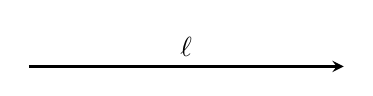
\begin{tikzpicture}[>=stealth]
\draw[thick,->](0,0)--node[above]{$\ell$}(4,0);
\end{tikzpicture}    
\captionof{figure}{ }
\end{minipage}\hfill
\begin{minipage}{.45\textwidth}
\centering
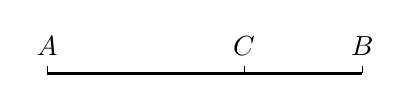
\begin{tikzpicture}
\draw[thick](0,0)--(4,0);
\foreach \x/\y in {0/A, 2.5/C, 4/B}
{
    \draw(\x,0)--(\x,.1)node[above]{$\y$};
}
\end{tikzpicture}    
\captionof{figure}{ }
\end{minipage}

\subsection{有向线段}
在物理学中，我们学过位移、速度、加速度等矢量，矢量的数学模型就是有向线段.规定了方向，即规定了起点和终点的线段叫做\textbf{有向线段}．如图1.2中的线段$AB$，如果以$A$为起点、$B$为终点，那么，它的方向是从$A$到$B$；相反，如果以$B$为起点、$A$为终点，它的方向就是从$B$到$A$. 表示有向线段时，要将表示起点的字母写在前面，表示终点的字母写在后面. 如以$A$为起点、$B$为终点的有向线段记作$\overline{AB}$. 图1.2中，点$C$是线段$AB$上的一点，$\overline{AB}$和$\overline{AC}$是方向相同的有向线段，$\overline{AB}$和$\overline{BC}$是方向相反的有向线段.

如果有向线段在有向直线$\ell$上或与$\ell$平行，那么，它的方向与$\ell$的正方向可能相同或相反．例如图1.3中的$\overline{AB}$与$\ell$的方向相同，而$\overline{BA}$与$\ell$的方向相反.

\noindent
\begin{minipage}{.45\textwidth}
\centering
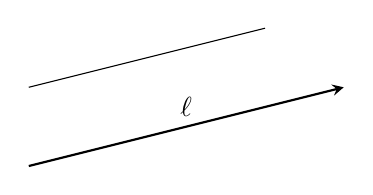
\begin{tikzpicture}[>=stealth]
\draw[thick,->](0,0)--node[above]{$\ell$}(4,1);
\draw(0,1)--(3,3/4+1);
\tkzDefPoints{1/1.25/A, 2.5/1.625/B}
\tkzLabelPoints[above](A,B)
\tkzDrawPoints(A,B)

\end{tikzpicture}    
\captionof{figure}{ }
\end{minipage}\hfill
\begin{minipage}{.45\textwidth}
\centering
\begin{tikzpicture}
\draw[thick, ->](0,0)--(4,0);
\foreach \x/\y in {1.5/A, 3/B}
{
    \draw(\x,0)--(\x,.1)node[above]{$\y$};
}
\draw[|-|](1.25,1.5)--node[above]{$e$}(1.75,1.5);
\end{tikzpicture}    
\captionof{figure}{ }
\end{minipage}




\subsection{有向线段的数量}
选定一条线段作为长度单位，我们可以量得一条线段的长度，线段$AB$的长度，就是有向线段$\overline{AB}$的长度，记作$|AB|$. 如图1.4中，设线段$e$为长度单位，那么$|AB|=3$. 因为有向线段的长度与它的方向无关，所以$|AB|=|BA|$.

根据$\overline{AB}$与有向直线$\ell$的方向相同或相反，分别把它的长度加上正号或负号，这样所得的数，叫做有向线段的\textbf{数量}（或\textbf{数值}）. 有向线段$\overline{AB}$的数量用$AB$表示\footnote{在引入有向直线以后，线段$AB$的长度一律用$|AB|$表示.}.显然
\[AB=-BA\]
也可写成
\[AB+BA=0\]

\section{直线上的坐标系——数轴}
\subsection{数轴上点的坐标}
在初中我们学过数轴，数轴上点的位置由一个实数（即坐标）唯一确定. 事实上数轴上点$P$的坐标$x_0$是以有向线段的数量来定义的. 点$P$的坐标$x_0$规定为有向线段$\overline{OP}$的数量，
即$OP=x_0$. 例如，点$A$、$B$的坐标分别是有向线段$OB$的数量，$x_A=OA=3$、$x_B=OB=-2$（图1.5）．
这样，数轴上的点和实数间建立了一一对应的关系.
\begin{figure}[htp]
    \centering
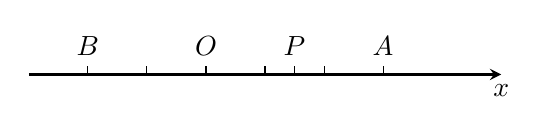
\begin{tikzpicture}[>=stealth, scale=.75]
\draw[->, thick](-3,0)--(5,0)node[below]{$x$};
\foreach \x in {-2,-1,...,3, 1.5}
{
    \draw(\x,0)--(\x,.15);
}
\foreach \x/\y in{-2/B, 0/O, 1.5/P, 3/A}
{
    \node at (\x,.15)[above]{$\y$};
}

\end{tikzpicture}
    \caption{}
\end{figure}

\subsection{数轴上有向线段的数量和两点距离公式}

\noindent
\begin{minipage}{.45\textwidth}
\CTEXindent
对于数轴上任意一条有向线段，它的数量显然与它的起点和终点的位置有关，也就是说与起点和终点的坐标有关. 从图1.6(1)中不难得到$AB=x_B-x_A$. 这个结论是否对任意的有向线段都成立呢？于是有如下猜想：

设$\overline{AB}$为$x$轴上任意一条有向线段，$O$是原点，点$A$、$B$的坐标分别为$x_1$、$x_2$，那么有
\[AB=x_2-x_1\]    
\end{minipage}\hfill
\begin{minipage}{.45\textwidth}
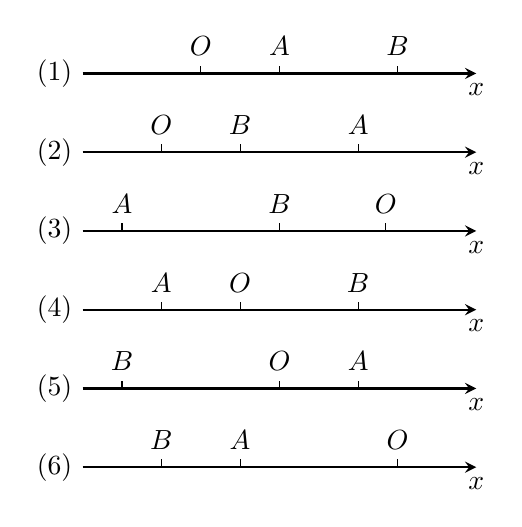
\begin{tikzpicture}[>=stealth]
\begin{scope}
    \draw[->,  thick](0,0)node[left]{(1)}--(5,0)node[below]{$x$};
\foreach \x/\y in {1.5/O,2.5/A,4/B}
{
    \draw(\x, 0)--(\x,.1)node[above]{$\y$};
}

\end{scope}  
\begin{scope}[yshift=-1cm]
    \draw[->,  thick](0,0)node[left]{(2)}--(5,0)node[below]{$x$};
\foreach \x/\y in {1/O,2/B,3.5/A}
{
    \draw(\x, 0)--(\x,.1)node[above]{$\y$};
}

\end{scope} 
\begin{scope}[yshift=-2cm]
    \draw[->,  thick](0,0)node[left]{(3)}--(5,0)node[below]{$x$};
\foreach \x/\y in {3.85/O,.5/A,2.5/B}
{
    \draw(\x, 0)--(\x,.1)node[above]{$\y$};
}

\end{scope} 
\begin{scope}[yshift=-3cm]
    \draw[->,  thick](0,0)node[left]{(4)}--(5,0)node[below]{$x$};
\foreach \x/\y in {1/A,2/O,3.5/B}
{
    \draw(\x, 0)--(\x,.1)node[above]{$\y$};
}

\end{scope} 
\begin{scope}[yshift=-4cm]
    \draw[->,  thick](0,0)node[left]{(5)}--(5,0)node[below]{$x$};
\foreach \x/\y in {.5/B,2.5/O,3.5/A}
{
    \draw(\x, 0)--(\x,.1)node[above]{$\y$};
}

\end{scope} 
\begin{scope}[yshift=-5cm]
    \draw[->,  thick](0,0)node[left]{(6)}--(5,0)node[below]{$x$};
\foreach \x/\y in {1/B,2/A,4/O}
{
    \draw(\x, 0)--(\x,.1)node[above]{$\y$};
}

\end{scope} 
\end{tikzpicture}    
\captionof{figure}{}
\end{minipage}


\begin{analyze}
由于$OA=x_1$、$OB=x_2$，所以需要证明$AB=OB-OA$. 当$A$、$B$和$O$都不重合时，它们的位置关系不同，证明方法也不尽相同，因此要先讨论它们的位置关系，然后再分情况进行论证.
\end{analyze}

\begin{proof}
当$A$、$B$和原点$O$都不重合时，在数轴上的相对位置共有六种，如图1.6所示．现就情况（4）进行证明．

$\because\quad AB=|AB|,\quad OA=-|OA|,\quad OB=|OB|$

又$\because\quad |AB|=|OA|+|OB|$

$\therefore\quad AB=OB-OA=x_2-x_1$

同理可证，对于其他五种情况等式也成立.

容易验证，当点$A$或点$B$与原点$O$重合时，这个等式同样成立.
\end{proof}

这样，我们就得到
\begin{thm}
    {定理} $\overline{AB}$为$x$轴上任意一条有向线段，点$A$、$B$的坐标分别为$x_1$、$x_2$，则有
\[AB=x_2-x_1\]
\end{thm}

根据这个定理可以得到，数轴上两点$A$、$B$的距离公式
\[|AB|=|x_2-x_1|\]

\begin{example}
    $A$、$B$、$C$为有向直线上任意三点，求证：
$AC=AB+BC$
\end{example}

\begin{analyze}
 如果在有向直线上建立数轴，那么有向线段数量问题就可以转化为代数问题.
\end{analyze}

\begin{proof}
在有向直线上建立数轴，设点$A$、$B$、$C$的坐标分别为$x_1$、$x_2$、$x_3$，则
\[AC=x_3-x_1,\qquad AB+BC=(x_2-x_1)+(x_3-x_2)=x_3-x_1\] 

$\therefore\quad AC=AB+BC$

关系式也可写成$AB+BC=AC$，通常称为数轴上有向线段的加法定理.

\end{proof}

\subsection{线段的定比分点}
有向直线$\ell$上的一点$P$，把$\ell$上的有向线段$\overline{P_1P_2}$分成两条有向线段$\overline{P_1P}$和$\overline{PP_2}$. $\overline{P_1P}$和$\overline{PP_2}$数量的比叫做点$P$分$\overline{P_1P_2}$所成的比，通常用字母$\lambda$来表示，即
\[\lambda=\frac{P_1P}{PP_2}\]
点$P$叫做$\overline{P_1P_2}$的定比分点。

\noindent
\begin{minipage}{.55\textwidth}
 \CTEXindent   如果点$P$在线段$P_1P_2$上（图1.7甲），点$P$叫做$P_1P_2$的\textbf{内分点}. 这时，无论$\ell$的方向如何，$\overline{P_1P}$和$\overline{PP_2}$的方向都相同，它们的数量的符号也相同，所以$\lambda$为正值. 如果点$P$在线段$P_2P_1$或$P_1P_2$的延长线上（图1.7乙、丙），点$P$叫做$\overline{P_1P_2}$的\textbf{外分点}. 这时无论$\ell$的方向如何，$\overline{P_1P}$和$\overline{PP_2}$的方向都相反，它们的数量的符号也相反，所以$\lambda$为负值.
\end{minipage}\hfill
\begin{minipage}{.4\textwidth}
\begin{tikzpicture}[>=stealth]
\begin{scope}
\draw[thick,->](0,0)node[left]{甲}--(4.5,0);
\foreach \x/\y in {1/P_1,1.8/P,3.5/P_2}
{
    \draw(\x,0)--(\x,.1)node[above]{$\y$};
}

\end{scope}
\begin{scope}[yshift=-1.5cm]
\draw[thick,->](0,0)node[left]{乙}--(4.5,0);
\foreach \x/\y in {.5/P,1.5/P_1,3.5/P_2}
{
    \draw(\x,0)--(\x,.1)node[above]{$\y$};
}

\end{scope}
\begin{scope}[yshift=-3cm]
\draw[thick,->](0,0)node[left]{丙}--(4.5,0);
\foreach \x/\y in {1/P_1,2.5/P_2,3.5/P}
{
    \draw(\x,0)--(\x,.1)node[above]{$\y$};
}

\end{scope}
\end{tikzpicture}
\captionof{figure}{}
\end{minipage}


由于点$P$分$\overline{P_1P_2}$所成的比与它们所在的直线$\ell$的方向
无关，为了简便起见，在以后谈到点$P$分$\overline{P_1P_2}$所成的比时，一般不提它所在的有向直线的方向.

\begin{thm}
    {思考题}讨论点$P$分$\overline{P_1P_2}$的比$\lambda$的取值范围；$P$在$\overline{P_1P_2}$所在有向直线上运动时，$\lambda$取值的变化情况.
\end{thm}

\subsection{数轴上线段的定比分点坐标公式}
设$P_1$、$P_2$是数轴上的两个已知点，其坐标分别是$x_1$、$x_2$，$\lambda$是已知实数且$\lambda\ne -1$，试在数轴上找一点$P$，使$\frac{P_1P}{PP_2}=\lambda$.

\begin{analyze}
    要找点$P$，只要求出点$P$的坐标.
\end{analyze}

\begin{solution}
设点$P$的坐标为$x$，则
\[P_1P=x-x_1,\qquad PP_2=x_2-x\]
要使$\frac{P_1P}{PP_2}=\lambda$，只要$\frac{x-x_1}{x_2-x}=\lambda$，解方程得
\[x=\frac{x_1+\lambda x_2}{1+\lambda}\quad (\lambda\ne -1)\]
\end{solution}

此公式叫做数轴上有向线段的定比分点坐标公式. 在运用这个公式时，一定要注意$x_1$是起点坐标，$x_2$是终点坐标.

当点$P$是线段$\overline{P_1P_2}$的中点时，有$P_1P=PP_2$，即$\lambda=1$. 因此线段$\overline{P_1P_2}$的中点$P$的坐标是
\[x=\frac{x_1+x_2}{2}\] 

\begin{example}
    若数轴上两个点$P_1$、$P_2$的坐标分别是$x_1=3$, $x_2=-2$，点$P$分$\overline{P_1P_2}$所成的比$\lambda=\frac{1}{3}$，试求分点$P$的坐标.
\end{example}

\begin{solution}
    由定比分点公式，可得
\[x=\frac{x_1+\lambda x_2}{1+\lambda}=\frac{3+\frac{1}{3}(-2)}{1+\frac{1}{3}}=\frac{9-2}{3+1}=\frac{7}{4}\]
\end{solution}

\begin{example}
若数轴上两个点$P_1$、$P_2$的坐标分别是$x_1=4$, $x_2=-2$，点$P$到$P_2$的距离为$|P_1P_2|$的一半，求线段$\overline{P_1P_2}$的分点$P$的坐标.
\end{example}

\begin{analyze}
    此题没有直接给出分比$\lambda$的数值. 自然，应该先求出$\lambda$，然后再用定比分点坐标公式去算分点坐标.
\end{analyze}

\begin{solution}
    \textbf{解法1：}为求$\lambda$的值，可画出草图分析分点$P$的位置（图1.8）．
\begin{figure}[htp]
    \centering
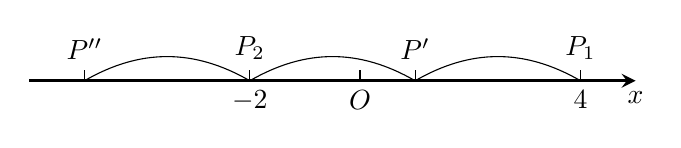
\begin{tikzpicture}[>=stealth, scale=.7]
    \draw[->, very thick](-6,0)--(5,0)node[below]{$x$};
\foreach \x/\y in {-5/P'',-2/P_2,1/P',4/P_1}
{
    \draw(\x,0)--(\x,.2)node[above]{$\y$};
}
\foreach \x in {-2,4}
{
    \node at (\x,0)[below]{$\x$};
}
\draw (0,0) node[below]{$O$}--(0,.2);

\draw(-5,0)[bend left=30] to (-2,0)[bend left=30] to (1,0)[bend left=30] to (4,0);

\end{tikzpicture}

    \caption{}
\end{figure}

由于$|PP_2|=\frac{1}{2}|P_1P_2|$，可能有一个内分点$P'$，还可能有一个外分点$P''$.

设$\lambda$为点$P$分$\overline{P_1P_2}$的比，此时，
\begin{enumerate}[(1)]
    \item $P$为内分点，即为点$P'$，

$\because\quad    |P'P_2|=\frac{1}{2}|P_1P_2|, \quad \lambda'=\frac{P_1P'}{P'P_2}=1$,

$\therefore\quad x'=\frac{x_1+x_2}{2}=\frac{4+(-2)}{2}=1$

\item $P$为外分点，即为点$P''$，

$\because\quad |P''P_2|=\frac{1}{2}|P_1P_2|,\quad \lambda''=\frac{P_1P''}{P''P_2}=\frac{-3}{1}=-3$

$\therefore\quad x''=\frac{4+(-3)(-2)}{1+(-3)}=-5$

$\therefore\quad $分点$P$的坐标为1或$-5$.
\end{enumerate}

\textbf{解法2：}设点$P$的坐标为$x$，

$\because\quad |PP_2|=\frac{1}{2}|P_1P_2|$

$\therefore\quad |(-2)-x|=\frac{1}{2}|(-2)-4|\Rightarrow |x+2|=3\Rightarrow x+2=\pm 3$

$\therefore\quad x=1$或$x=-5$

$\therefore\quad $分点$P$的坐标为1或$-5$.
\end{solution}

\begin{ex}
\begin{enumerate}
    \item 填空题：若数轴上点$A$、$B$、$C$的坐标分别是$\sin^2\alpha$、$-\cos^2\alpha$、$-1$
\begin{enumerate}[(1)]
    \item $AB=\blank$；$BC=\blank$；$CO=\blank$；
    \item $|AB|=\blank$；$|BC|=\blank$；$|CO|=\blank$；
    \item $M$是数轴上一点，且$CM=-5$，$M$点的坐标是\blank;
    \item $N$是数轴上一点，且$|AN|=1-\cos^2\alpha$，$N$的坐标是\blank.
\end{enumerate}
\item 填空题：若$|P_1P_2|=5$，点$P$分$\overline{P_1P_2}$的定比为$\lambda$，
\begin{enumerate}[(1)]
    \item 点$P$在线段$P_1P_2$上，且$|P_1P|=2$, $\lambda=\blank$;
    \item  点$P$在线段$P_1P_2$的延长线上，且$|PP_2|=3$, $\lambda=\blank$;
    \item 点$P$在线段$P_2P_1$的延长线上，且$|PP_1|=3$, $\lambda=\blank$;
\end{enumerate}
\item 填空题：若点$C$分$\overline{AB}$所成的比为2，则点$B$分$\overline{AC}$所成的比$=\blank$；点$A$分$\overline{BC}$所成的比$=\blank$；点$A$分$\overline{CB}$所成的比$=\blank$.
\item 已知点$A$、$B$的坐标分别是$-2$和4，点$M$分$\overline{AB}$所成的比为$\lambda$，按照下面所给$\lambda$的值，求点$M$的坐标：
\begin{multicols}{3}
\begin{enumerate}[(1)]
    \item $\lambda= 1$
    \item $\lambda= \frac{1}{3}$
    \item $\lambda= -3$
    \item $\lambda= 0$
    \item $\lambda= -0.25$
\end{enumerate}
\end{multicols}
\end{enumerate}
\end{ex}

\section{平面上的坐标系——直角坐标系和极坐标系}

\noindent
\begin{minipage}{.65\textwidth}
    \CTEXindent
在初中，我们学过直角坐标系. 在直角坐标平面内，任一点$P$的位置由一对有序实数$(x,y)$唯一确定. 其中$x$为点$P$在$x$轴上射影$M$的坐标，$y$为点$P$在$y$轴上射影$N$的坐标（图1.9）．这样，坐标平面$xOy$上的点就与有序实数对$(x,y)$之间建立了一一对应的关系.    
\end{minipage}\hfill
\begin{minipage}{.32\textwidth}
\centering
\begin{tikzpicture}[>=stealth, scale=.9]
\draw[->](-1,0)--(3,0)node[below]{$x$};
\draw[->](0,-.5)--(0,3)node[left]{$y$};
\draw[dashed](0,2)node[left]{$N$}--(1.5,2)node[right]{$P$}--(1.5,0)node[below]{$M$};
\node [below left]{$O$};
\draw[fill](1.5,2) circle (1.5pt);
\end{tikzpicture}
\captionof{figure}{}
\end{minipage}

确定平面上点的位置，除了直角坐标系的方法外，还可采取极坐标系的办法. 极坐标系将在第五章中专门介绍.


\subsection{平面内两点距离公式}

在直角坐标系中，已知两点$P_1(x_1,y_1)$、$P_2(x_2,y_2)$，试求$P_1$、$P_2$的距离$|P_1P_2|$.

\begin{analyze}
    平面上点$P$的横、纵坐标是借助数轴上点（即点$P$在$x$轴、$y$轴上射影）的坐标来定义的；而数轴上两点间的距离公式又是我们已经熟悉的.因此，很自然地想到把问题转化为数轴上的问题加以解决.
\end{analyze}

\begin{solution}
\begin{enumerate}[(1)]
\noindent
\begin{minipage}{.45\textwidth}
 \item 当$P_1P_2\parallel x$轴时（图1.10），分别作$P_1$、$P_2$在$x$轴上的射影$M_1$、$M_2$，则$M_1(x_1,0)$、$M_2(x_2,0)$
    
 $\therefore\quad    |P_1P_2|=|M_1M_2|=|x_2-x_1|$


 \item 当$P_1P_2\parallel y$轴，同理可得$|P_1P_2|=|y_2-y_1|$.    
\end{minipage}\hfill
\begin{minipage}{.45\textwidth}
\centering
\begin{tikzpicture}[>=stealth]
    \draw[->](-3,0)--(2,0)node[below]{$x$};
    \draw[->](0,-.5)--(0,3)node[left]{$y$};
    \draw[dashed](-2,0)node[below]{$M_1$}--(-2,2)node[above]{$P_1$};
    \draw[dashed](1,0)node[below]{$M_2$}--(1,2)node[above]{$P_2$};
    \draw[thick](-2,2)--(1,2);
    \node [below left]{$O$};
    \foreach \x in {-2,1}
    {
        \draw[fill](\x,2) circle (1.5pt);
    }
\end{tikzpicture}
\captionof{figure}{}
\end{minipage}

\begin{minipage}{.45\textwidth}
\item  当$P_1P_2\not\parallel x$轴且$P_1P_2\not\parallel y$轴时（图1.11），分别过点$P_1$、$P_2$作$x$轴和$y$轴的垂线并延长相交于$Q$，则点$Q$的坐标为$(x_1,y_2)$.

$\because\quad P_1Q\parallel y$轴，

$\therefore\quad |P_1Q|=|y_2-y_1|$,

又$\because\quad P_2Q\parallel x$轴，

$\therefore\quad |P_2Q|=|x_2-x_1|$, 

在${\rm Rt}\triangle P_1QP_2$中，
\[\begin{split}
    |P_1P_2|^2&=|P_1Q|^2+|P_2Q|^2\\
    &=|y_2-y_1|^2+|x_2-x_1|^2
\end{split}\]
\end{minipage}\hfill
\begin{minipage}{.45\textwidth}
\centering
\begin{tikzpicture}[>=stealth]
    \draw[->](-2.5,0)--(2.5,0)node[below]{$x$};
    \draw[->](0,-2)--(0,3)node[left]{$y$};
    \draw[dashed](-1.5,-1)node[below]{$Q$}--(-1.5,2)node[above]{$P_1$};
    \draw[dashed](-1.5,-1)--(1.5,-1)node[below]{$P_2$};
    \draw[thick](-1.5,2)--(1.5,-1);
    \node [below left]{$O$};
    \foreach \x/\y in {-1.5/-1, -1.5/2, 1.5/-1}
    {
        \draw[fill](\x,\y) circle (1.5pt);
    }
\end{tikzpicture}
\captionof{figure}{}
\end{minipage}

$\therefore\quad |P_1P_2|=\sqrt{(x_2-x_1)^2+(y_2-y_1)^2}$
\end{enumerate}    
\end{solution}

很明显，（1）、（2）是（3）的特殊情况，公式对（1）、（2）同样适用．这样，我们就得到了平面上两点间的距离公式：
\[|P_1P_2|=\sqrt{(x_2-x_1)^2+(y_2-y_1)^2}\]





\begin{example}
$\triangle ABC$中，$AO$是$BC$边上的中线，求证：
\[|AB|^2+|AC|^2=2(|AO|^2+|OC|^2)\]
\end{example}

\begin{analyze}
这是一个平面几何问题，当然可用平面几何的方法证明.现在我们借助坐标系，用代数的方法证明，以理解平面解析几何的基本思想.
\end{analyze}

\begin{proof}

\noindent
\begin{minipage}{.55\textwidth}
\CTEXindent 取线段$BC$所在直线为$x$轴，点$O$为原点建立直角坐标系，如图1.12．

设点$A$的坐标为$(b,c)$，点$C$的坐标为$(a,0)$，则点$B$的坐标为$(-a,0)$，可得
\[\begin{split}
|AB|^2&=(a+b)^2+c^2,\\
|AC|^2&=(a-b)^2+c^2,\\
|AO|^2&=b^2+c^2,\quad |OC|^2=a^2.    
\end{split}\]    
\end{minipage}\hfill
\begin{minipage}{.45\textwidth}
\centering
\begin{tikzpicture}[>=stealth]
    \draw[->](-2.5,0)--(2.5,0)node[below]{$x$};
    \draw[->](0,-1)--(0,2.5)node[left]{$y$};
    \tkzDefPoints{-1.5/0/B, 0/0/O, 1.5/0/C, 1/1.5/A}
\draw(A)--(B);
\draw(A)--(O);
\draw(A)--(C);
\tkzLabelPoints[below](B,C)
\tkzLabelPoints[below left](O)
\tkzLabelPoints[above](A)

\end{tikzpicture}
\captionof{figure}{}
\end{minipage}

$\therefore\quad |AB|^2+|AC|^2=2(a^2+b^2+c^2),\quad |AO|^2+|OC|^2=a^2+b^2+c^2$

$\therefore\quad |AB|^2+|AC|^2=2(|AO|^2+|OC|^2)$.
\end{proof}

\begin{example}
若$a,b,c,d\in\R$，求证：
$$\sqrt{a^2+b^2}+\sqrt{c^2+d^2}\ge \sqrt{(a-c)^2+(b-d)^2}$$
\end{example}

\begin{analyze}
    这是一个代数问题，当然可用代数方法证明. 我们能不能借助坐标系，把它转化为几何问题，用几何方法给以证明呢？这里，关键是找到根式$\sqrt{a^2+b^2}$，$\sqrt{c^2+d^2}$，$\sqrt{(a-c)^2+(b-d)^2}$的几何形式.
\end{analyze}

\begin{proof}
建立直角坐标系$xOy$，取点$A(a,b)$、点$B(c,d)$（图1.13），则有
$$\sqrt{a^2+b^2}=|AO|,\quad \sqrt{c^2+d^2}=|BO|,\quad \sqrt{(a-c)^2+(b-d)^2}=|AB|$$
所以只需证
\[|AO|+|BO|\ge |AB|\]

\begin{enumerate}[(1)]
    \item 当$A$、$B$、$O$三点不共线时，根据三角形性质可知：
    \[|AO|+|BO|> |AB|\]
\begin{minipage}{.55\textwidth}

\item 当$A$、$B$、$O$三点共线时，
\begin{itemize}
    \item 若点$A$、$B$在点$O$同侧，包括$A$、$B$重合，都有
\[|AO|+|BO|>|AB|\]
\item 若点$A$、$B$在点$O$的两侧，则有
\[|AO|+|BO|=|AB|\]    
\end{itemize}
\end{minipage}\hfill
\begin{minipage}{.45\textwidth}
\centering
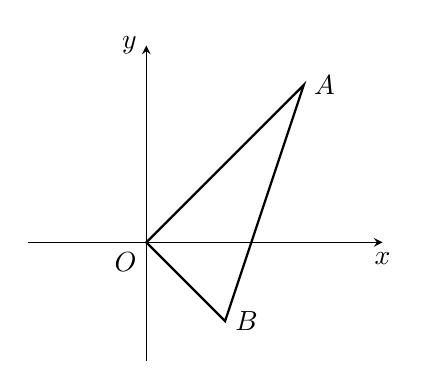
\begin{tikzpicture}[>=stealth]
\draw[->](-1.5,0)--(3,0)node[below]{$x$};    
\draw[->](0,-1.5)--(0,2.5)node[left]{$y$}; 
\node[below left]{$O$};
\draw[thick](0,0)--(2,2)node[right]{$A$}--(1,-1)node[right]{$B$}--cycle;   
\end{tikzpicture}
\captionof{figure}{}
\end{minipage}
\begin{itemize}
\item 若点$A$、$B$中有且只有一个点与点$O$重合，不妨设点$B$与点$O$重合，则有
\[|AO|+|BO|=|AO|=|AB|\]
\item 若点$A$、$B$都与点$O$重合，则
\[|AO|+|BO|=|AB|=0\]
\end{itemize}
$\therefore\quad $对$a,b,c,d\in\R$，不等式
$\sqrt{a^2+b^2}+\sqrt{c^2+d^2}\ge \sqrt{(a-c)^2+(b-d)^2}$恒成立.

\end{enumerate}    
\end{proof}

通过例1.4、例1.5可以看到，建立坐标系后，几何问题与代数问题的互化有了基础，这就为找到简捷优美的解题方法创造了条件，这正是解析几何学基本思想的体现.

\subsection{平面内线段定比分点坐标公式}
若$P_1(x_1,y_1)$、$P_2(x_2,y_2)$是平面上两个已知点，在线段$\overline{P_1P_2}$所在直线上找一点$P$，使得
\[\frac{P_1P}{PP_2}=\lambda\quad (\lambda\in\R,\; \lambda\ne -1)\]
 
\begin{analyze}
    求点$P$即求点$P$的坐标. 上节我们已解决了数轴上求线段的定比分点坐标问题，现在是求平面内线段定比分点的坐标. 同样由于平面内点的坐标是借助数轴上点的坐标定义的，因此平面内的线段定比分点问题可以转化为数轴上的相应问题加以解决.
\end{analyze}

\begin{solution}
设点$P$的坐标为$(x,y)$，过点$P_1$、$P_2$、$P$分别作$x$轴的垂线$P_1M_1$、$P_2M_2$、$PM$，则垂足分别为$M_1(x_1,0)$、$M_2(x_2,0)$、$M(x,0)$（图1.14）．根据平行线截割定理，得

\noindent
\begin{minipage}{.5\textwidth}
\[\frac{|P_1P|}{|PP_2|}=\frac{|M_1M|}{|MM_2|}\]

\CTEXindent 如果点$P$在线段$P_1P_2$上，那么点$M$也在线段$M_1M_2$上；如果点$P$在线段$P_1P_2$或线段$P_2P_1$的延长线上，那么点$M$也在线段$M_1M_2$或$M_2M_1$的延长线上. 因此，$\frac{P_1P}{PP_2}$与$\frac{M_1M}{MM_2}$的符号相同，所以
    \[\frac{P_1P}{PP_2}=\frac{M_1M}{MM_2}\]    
\end{minipage}\hfill
\begin{minipage}{.45\textwidth}
\centering
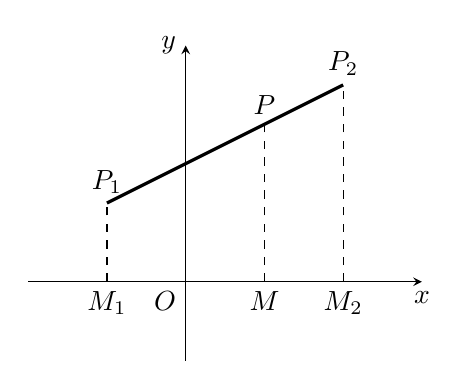
\begin{tikzpicture}[>=stealth]
    \draw[->](-2,0)--(3,0)node[below]{$x$};    
\draw[->](0,-1)--(0,3)node[left]{$y$}; 
\node[below left]{$O$};
\draw[dashed](-1,0)node[below]{$M_1$}--(-1,1)node[above]{$P_1$};
\draw[dashed](1,0)node[below]{$M$}--(1,2)node[above]{$P$};
\draw[dashed](2,0)node[below]{$M_2$}--(2,2.5)node[above]{$P_2$};
\draw[very thick](-1,1)--(2,2.5);
\end{tikzpicture}
\captionof{figure}{}
\end{minipage}

$\because\quad \frac{P_1P}{PP_2}=\lambda, \qquad \qquad \therefore\quad \frac{M_1M}{MM_2}=\lambda$.

这样，就把平面上的问题转化为数轴上的问题. 根据上节的结论，得
\[x=\frac{x_1+\lambda x_2}{1+\lambda}\]
同理可以求得
\[y=\frac{y_1+\lambda y_2}{1+\lambda}\]
\end{solution}

因此，当已知$P_1(x_1,y_1)$、$P_2(x_2,y_2)$，点$P(x,y)$分线段$\overline{P_1P_2}$所成的比为$\lambda\; (\lambda\in\R,\; \lambda\ne -1)$时，点$P$的坐标是
\[x=\frac{x_1+\lambda x_2}{1+\lambda},\qquad y=\frac{y_1+\lambda y_2}{1+\lambda}\]

和上节一样，当$P$是线段$\overline{P_1P_2}$的中点时，有$P_1P=PP_2$，即$\lambda=1$. 因此线段$\overline{P_1P_2}$中点$P$的坐标是
\[x=\frac{x_1+x_2}{2},\qquad y=\frac{y_1+y_2}{2}\]

\begin{example}
已知$P_1(-1,-6)$，$P_2(3,0)$，反向延长$P_1P_2$到$P$，使$|P_1P|=\frac{1}{3}|P_1P_2|$，求线段$P_1P_2$的分点$P$的坐标.
\end{example}

\begin{solution}
    \textbf{解法1：} 作图1.15．设点$P$的坐标为$(x,y)$, $\lambda=\frac{P_1P}{PP_2}$, 则有

\noindent
\begin{minipage}{.55\textwidth}
\[\begin{split}
\lambda&=\frac{1}{4}\\
x&=\frac{-1+\left(-\frac{1}{4}\right)\cdot 3}{1+\left(-\frac{1}{4}\right)}=-\frac{7}{3}\\
y&=\frac{-6+\left(-\frac{1}{4}\right)\cdot 0}{1+\left(-\frac{1}{4}\right)}=-8
\end{split}\]

$\therefore\quad $点$P$的坐标是$\left(-\frac{7}{3},-8\right)$
\end{minipage}\hfill
\begin{minipage}{.45\textwidth}
\centering
\begin{tikzpicture}[>=stealth, scale=.6]
    \draw[->](-4,0)--(4,0)node[below]{$x$};    
\draw[->](0,-8)--(0,1)node[left]{$y$}; 
\node[below left]{$O$};
\draw[thick](-7/3,-8)node[left]{$P$}--(3,0)node[above]{$P_2$};
\draw[fill](-7/3,-8) circle(1.5pt);
\draw[fill](-1,-6)node[left]{$P_1$} circle(1.5pt);
\node at (3,0)[below]{3};
\draw(0,-6)--(.1,-6)node[right]{$-6$};

\end{tikzpicture}
\captionof{figure}{}
\end{minipage}

\textbf{解法2：}设$\lambda=\frac{P_2P_1}{P_1P}$，则$\lambda=3$，

$\because\quad -1=\frac{3+3x}{1+3},\qquad \qquad \therefore\quad x=-\frac{7}{3}$

$\because\quad -6=\frac{0+3y}{1+3},\qquad \qquad \therefore\quad y=-8$

$\therefore\quad $点$P$的坐标是$\left(-\frac{7}{3},-8\right)$
\end{solution}

由此可见，用定比分点坐标公式可以灵活地重新选定起点、终点和分点. 一旦选定，$\lambda$也就随之而定. 因此解题时，必须说明$\lambda$的意义.

\begin{example}
    三角形重心坐标公式．
已知三角形顶点是$A(x_1,y_1)$，$B(x_2,y_2)$，$C(x_3,y_3)$，求$\triangle ABC$的重心$G$的坐标$(x,y)$（图1.16）．
\end{example}

\begin{solution}
设$BC$边的中点为$D$，则点$D$的坐标是$\left(\frac{x_2+x_3}{2},\; \frac{y_2+y_3}{2}\right)$

\noindent
\begin{minipage}{.55\textwidth}
又因为$AD$是中线，且$\frac{AG}{GD}=2$，所以点$G$的坐标是
\[\begin{split}
    x&=\frac{x_1+2\x \frac{x_2+x_3}{2}}{1+2}\\
    y&=\frac{y_1+2\x \frac{y_2+y_3}{2}}{1+2}
\end{split}\]
整理后得重心$G$的坐标
    \[x=\frac{x_1+x_2+x_3}{3},\quad y=\frac{y_1+y_2+y_3}{3}\]    
\end{minipage}\hfill
\begin{minipage}{.45\textwidth}
\centering
\begin{tikzpicture}[>=stealth]
\draw[->](-3,0)--(3,0)node[below]{$x$};    
\draw[->](0,-1.5)--(0,3.25)node[left]{$y$}; 
\node[above right]{$O$};
\tkzDefPoints{-2/-1/A, 2/.5/B, 1/3/C}
\tkzDefMidPoint(B,C) \tkzGetPoint{D}
\draw(A)--(B)--(C)--cycle;
\draw(A)--(D);
\tkzLabelPoints[right](B,C,D)
\tkzLabelPoints[below](A)
\tkzDefBarycentricPoint(A=1,D=2)
\tkzGetPoint{G}
\tkzLabelPoints[above](G)
\tkzDrawPoint(G)
\end{tikzpicture}
\captionof{figure}{}
\end{minipage}
\end{solution}

\begin{ex}
\begin{enumerate}
    \item 填空题：
\begin{enumerate}[(1)]
    \item $A(-2,3)$，$B(-4,-5)$，$|AB|=\blank$;
    \item $A\left(\frac{\sqrt{3}}{2},\; -\frac{\sqrt{2}}{2}\right)$，$B\left(-\frac{\sqrt{2}}{2},\; -\frac{\sqrt{3}}{2}\right)$，$|AB|=\blank$;
    \item $C(ab^2, 2abc)$，$D(ac^2,0)$，$|CD|=\blank$;
    \item $P_1(a\cos\alpha, a\sin\alpha)$，$P_2(a\sin\alpha,-a\cos\alpha)$，$|P_1P_2|=\blank$.
\end{enumerate}
    \item 已知两点$P_1(3,-2)$、$P_2(-9,4)$．求点$P(x,0)$分$\overline{P_1P_2}$所成的比$\lambda$及$x$的值.
    \item 点$M$分线段$\overline{M_1M_2}$的比为$\lambda$，求点$M$的坐标$(x,y)$:
\begin{enumerate}[(1)]
    \item 已知：$M_1(1,5)$、$M_2(2,3)$, $\lambda=\frac{1}{3}$
    \item 已知：$M_1(1,5)$、$M_2(2,3)$, $\lambda=-2$
    \item 已知：$M_1(1,5)$、$M_2(2,-3)$, $\lambda=-2$
\end{enumerate}
\item 已知$\triangle ABC$的顶点$A(2,3)$、$B(8,-4)$和重心$G(2,1)$. 求点$C$的坐标$(x,y)$.
\end{enumerate}
\end{ex}

\section*{习题一}
\begin{center}
    \bfseries A
\end{center}

\begin{enumerate}
\item 已知数轴上$A$、$B$两点的坐标$x_1$、$x_2$分别是：
\begin{multicols}{2}
\begin{enumerate}[(1)]
    \item $x_{1}= 5,\quad x_{2}= - 3$;
    \item $x_{1}= - 9,\quad x_{2}= - 11$;
    \item $x_{1}= 2a- b,\quad x_{2}= a- 2b$;
    \item $x_{1}= \sec ^{2}\alpha ,\quad x_{2}= 1$。
\end{enumerate}    
\end{multicols}
求$AB$.
\item $A$、$B$是数轴上两点，点$B$的坐标是$x_2$, 根据下列条件，
求点$A$的坐标$x_1$：
\begin{multicols}{2}
\begin{enumerate}[(1)]
    \item $x_{2}= 3,\quad | AB| = 5$;
    \item $x_{2}= - 5,\quad | AB| = 2$.
\end{enumerate}    
\end{multicols}

\item 求连结下列两点的线段的长度和中点坐标：
\begin{multicols}{2}
\begin{enumerate}[(1)]
    \item $P_{1}( 6, -4)$、$P_{2}( - 2, -2)$;
    \item $A(-2.8,6.4)$、$B(-2.8,7.2)$;
    \item $C(a\cos\theta,\; a\sin\theta)$、$D(0,0)$;
    \item $E( a, b) $、$F( - a$, $b) $.
\end{enumerate}
\end{multicols}
\item 一条线段的两个端点$P_1$、$P_2$的坐标及点$P$ 分$\overline {P_1 P_2}$所成的
比如下，求分点$P$的坐标：
\begin{multicols}{2}
\begin{enumerate}[(1)]
    \item $(5, -2),\quad (5, 3),\quad \lambda = - \frac 23$
    \item $(-4, 1),\quad (5, 4),\quad \lambda = \frac 52$
\end{enumerate}
\end{multicols}
\end{enumerate}

\begin{center}
    \bfseries B
\end{center}

\begin{enumerate}\setcounter{enumi}{4}
    \item $A$、 $B$、 $C$、 $D$是有向直线上的四个点，求证：
\begin{enumerate}[(1)]
    \item $AB\cdot CD+ BC\cdot AD= AC\cdot BD;$
    \item $AB+ BC+ CD+ DA= 0.$
\end{enumerate}
    \item 数 轴 上 三 点 $A$、$B$、 $C$ 的坐标分别是$-1$、5、3, 求这三点
    中每一点分其余两点间的线段所成的比.
    \item 已知点$P(x,2)$, $Q(-2,-3)$, $M(1,1)$, 且$|PQ|=|PM|$.
    求$x$.
    \item \begin{enumerate}[(1)]
        \item 求在$x$轴上与点$A(5,12)$的距离为13的点的坐标。
        \item 已知点$P$的横坐标是7，点$P$到点$N(-1,5)$的距离
    等于10，求点$P$的纵坐标。
    \end{enumerate}
    
    \item 已知$A(1,1),B(2,2),C(3,-1)$是一个平行四边形
    的三个顶点，求第四个顶点。
    \item \begin{enumerate}[(1)]
        \item 线段的两个端点的坐标是$(-1,2)$和$(-10,-1)$, 求
    这条线段的三等分点。
    \item 已知点$A(1,-1),B(-4,5)$,将线段$AB$延长至
    $C$,使$|AC|=3|AB|$, 求点$C$的坐标.
    \end{enumerate}
    \item 已知点$P_1(4,-3)$, $P_2(-2,6)$, 求适合下列条件的点
    $P$的坐标：
    \begin{enumerate}[(1)]
        \item $\frac {| P_{1}P| }{| PP_2 | }= 2$, 点$P$在线段$P_1P_2$上;
        \item $\frac {| P_{1}P| }{| PP_{2}| }= 4$, 点$P$ 在线段 $P_{1}P_{2}$的 延 长 线 上;
        \item $\frac {| P_{1}P| }{| PP_{2}| }= \frac 45$, 点$P$在线段$P_2P_{1}$的延长线上.
    \end{enumerate}
\item \begin{enumerate}[(1)]
    \item 已知三点$A(x,5)$、$B(-2,y)$、$C(1,1)$，且点$C$
平分线段$AB$. 求$x,y$.
\item 已知两点$A(3,-1)$、$B(2,1)$，求点$A$关于点$B$的对称点的坐标.
\end{enumerate} 
\item \begin{enumerate}[(1)]
    \item 证明：直角三角形斜边的中点到三个顶点的距离相等；
    \item 证明：三角形中位线等于底边的一半．
\end{enumerate}
\end{enumerate}

\begin{center}
    \bfseries C
\end{center}

\begin{enumerate}\setcounter{enumi}{13}
    \item 若点$P$分线段$AB$的比为$\lambda\; (\lambda\ne 1)$，求$A$分线段$PB$的比.
    \item 若$0<a<1$, $0<b<1$，试证明：
\[\sqrt{a^2+b^2}+\sqrt{(a-1)^2+b^2}+\sqrt{a^2+(b-1)^2}+\sqrt{(a-1)^2+(b-1)^2}\ge 2\sqrt{2}\]
\end{enumerate}


\section{曲线与方程的定义}
在前面，我们学习了点和坐标的知识，这就为研究曲线和方程提供了新的方法.

\noindent
\begin{minipage}{0.55\textwidth}
    \CTEXindent
17世纪初，人们对二元方程$f(x,y)=0$的认识还是初浅的. 认为二元方程的解是“不确定”的，故称它为“不定方程”. 例如二元一次方程$2x+y=0$，就有无数组解. 如果把$x$看作变量，对$x$在变化中取的每一个确定的值$x_1,x_2,\ldots, x_n,\ldots$，我们都可求出$y$的对应值$y_1,y_2,\ldots,y_n,\ldots$，对于$(x_1,y_1),\; (x_2,y_2),\; \ldots,(x_n,y_n),\; \ldots$，在直角坐标系中可得到对应的点，所有这些点的集合便构成一条曲线（图1.17）．这正是函数的最初的想法．    
\end{minipage}\hfill
\begin{minipage}{0.4\textwidth}
\centering
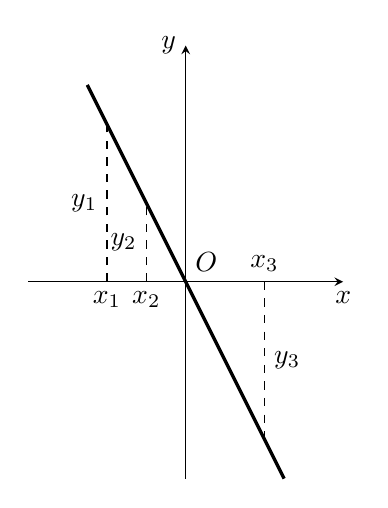
\begin{tikzpicture}[>=stealth]
\draw[->](-2,0)--(2,0)node[below]{$x$};
\draw[->](0,-2.5)--(0,3)node[left]{$y$};
\draw[very thick](-1.25,2.5)--(1.25,-2.5);
\node[above right]{$O$};
\draw[dashed](-.5,0)node[below]{$x_2$}--node[left]{$y_2$}(-.5,1);
\draw[dashed](-1,0)node[below]{$x_1$}--node[left]{$y_1$}(-1,2);
\draw[dashed](1,0)node[above]{$x_3$}--node[right]{$y_3$}(1,-2);

\end{tikzpicture}
\captionof{figure}{}
\end{minipage}




实际上，我们在初中学过正比例函数，函数$y=-2x$的图象是直线
$y=-2x$. 根据函数图象的概念可知：直线$y=-2x$上的点的坐标都满足函数关系$y=-2x$；反过来，坐标满足函数关系$y=-2x$的点都在直线$y=-2x$上. 从方程的角度看，方程$y+2x=0$与直线$y+2x=0$同样也有上述关系.

在初中，我们还学过函数$y=ax^2\; (a\ne 0)$的图象是关于$y$轴对称的抛物线. 根据函数图象的概念，如果把函数$y=ax^2$看作是方程$y=ax^2\; (a\ne 0)$，同样有：如果$M(x_0,y_0)$是抛物线上的点，那么$(x_0,y_0)$一定是这个方程的解；反过来，如果$(x_0,y_0)$是方程$y=ax^2\; (a\ne 0)$的解，那么以它为坐标的点一定在这条抛物线上. 这样，我们就说$y=ax^2\; (a\ne 0)$是这条抛物线的方程；抛物线是方程$y=ax^2\; (a\ne 0)$的曲线．

综上所述，我们把曲线$C$和方程$F(x,y)=0$的这种关系概括成

\subsection{曲线与方程的定义}
\begin{thm}
    {曲线与方程的定义}
在直角坐标系中，如果曲线$C$（适合某种条件的点的集合或轨迹）和方程$F(x,y)=0$满足如下关系：
\begin{enumerate}
    \item 曲线上的每一个点的坐标都是方程的实数解；
    \item 以方程的每一个实数解为坐标的点都在曲线上．
\end{enumerate}
那么，这个方程叫曲线$C$的方程；这条曲线叫方程$F(x,y)=0$的曲线（图形）. 简记为曲线$C:\; F(x,y)=0$.
\end{thm}

\begin{example}
    判断下列叙述是否正确，并说明理由：
\begin{enumerate}[(1)]
    \item “曲线$C$上无数个点的坐标都满足方程$F(x,y)=0$, 且方程$F(x,y)=0$的所有实数解为坐标的点都在曲线$C$上”，所以曲线$C$是方程$F(x,y)=0$的曲线.
    \item “三角形的一条中线上至少有两个点在$y$轴上，所以这条中线的方程是$x=0$.
\end{enumerate}
\end{example}

\begin{solution}
\begin{enumerate}[(1)]
\item 曲线$C$上无数点的坐标都满足方程$F(x,y)=0$，不能保证曲线$C$上每一个点的坐标都满足方程$F(x,y)=0$，这一点读者可举例说明. 因此，不满足曲线与方程定义的第一个条件，不能说曲线$C$是方程$F(x,y)=0$的曲线. 叙述不正确.
\item 三角线中线是一条线段，中线上两点在轴上，只说明中线在$y$轴上，但中线不是$y$轴. 因此，在三角形外的$y$轴上的点，它的坐标为$(0,y_0)$，满足方程$x=0$，但它不在中线上，不满足曲线与方程定义的第二个条件，所以不能说中线的方程为$x=0$. 叙述是不正确的.
\end{enumerate}
\end{solution}

\begin{example}
    证明方程$x^2+y^2=25$的曲线是以坐标原点为圆心，半径等于5的圆，并判断点$M_1(3,4)$，$M_2(-2\sqrt{5},2)$是否在这个圆上．
\end{example}

\begin{proof}
\begin{enumerate}[(1)]
    \item 设$M(x_0,y_0)$是圆上任意一点，因为点$M$到坐标原点的距离等于5，所以
    $\sqrt{x^2_0+y^2_0}=5$, 也就是$x^2_0+y^2_0=25$.
    即$(x_0,y_0)$是方程$x^2+y^2=25$的解.
    \item 设$(x_0,y_0)$是方程$x^2+y^2=25$的任一解，那么
    $x^2_0+y^2_0=25$.
    两边开方取算术根，得
    $\sqrt{x^2_0+y^2_0}=5$.
  即点$M(x_0,y_0)$到坐标原点的距离等于5，点$M(x_0,y_0)$是这个圆上的点.
\end{enumerate}    

\noindent
\begin{minipage}{.55\textwidth}
\CTEXindent 由（1）、（2）可知，$x^2+y^2=25$是以坐标原点为圆心，半径等于5的圆的方程．

把点$M_1(3,-4)$的坐标代入方程$x^2+y^2=25$，左右两边相等，$(3,-4)$是方程的解，所以点$M_1$在这个圆上；
    
把$M_2(-2\sqrt{5},2)$的坐标代入方程$x^2+y^2=25$，左右两边不等，$(-2\sqrt{5},2)$不是方程的解，所以点$M_2$不在这个圆上（如图1.18）．

\end{minipage}\hfill
\begin{minipage}{.4\textwidth}
\centering
\begin{tikzpicture}[>=stealth, scale=.3]
\draw[->](-7,0)--(7,0)node[below]{$x$};
\draw[->](0,-7)--(0,7)node[left]{$y$};
\node[below left]{$O$};
\draw(0,0) circle (5);
\tkzDefPoints{3/-4/M_1, -2*2.236/2/M_2}
\tkzLabelPoints[right](M_1,M_2)
\foreach \x in {1,2}
{
    \draw[fill](M_\x)circle (3pt);
}
\end{tikzpicture}
\captionof{figure}{}
\end{minipage}
\end{proof}    

通过上面例题，我们可以进一步理解曲线的方程或方程
的曲线的含义，这就是

曲线$C:\; F(x,y)=0$, 那么对点$P(x_0,y_0)$有
\[\begin{split}
    P(x_0,\:y_0) \in C&\Longleftrightarrow F(x_0,\:y_0)=0\\
P(x_0,\:y_0)\notin C&\Longleftrightarrow F(x_0,\:y_0)\ne 0
\end{split}\]

\subsection{曲线的公共点}

由曲线与方程的定义，不难得到有关曲线公共点的结论：

已知：曲线$C_1:\; F_1(x,y)=0$, 曲线$C_2:\; F_2(x,y)=0$,
则
\[P(x_{0},y_{0})\text{是$C_1,C_{2}$的公共点}\Longleftrightarrow\begin{cases}F_{1}(x_{0},y_{0})=0,\\F_{2}(x_{0},y_{0})=0.\end{cases}\]
读者可以证明这个结论.

由此可以知道，方程组有几组不同实数解，两条曲线就有几个公共点；方程组没有实数解，两条曲线就没有公共点.

\begin{example}
求直线$y=x+\frac{3}{2}$被曲线$y=\frac{1}{2}x^2$截得的线段的长.
\end{example}

\begin{solution}
先求公共点. 解方程组    

    \noindent
\begin{minipage}{.45\textwidth}
\[\begin{cases}
    y=x+\frac{3}{2}\\
    y=\frac{1}{2}x^2
\end{cases}\]
得
\[\begin{cases}
    x_1=-1\\
    y_1=\frac{1}{2}
\end{cases}\qquad \begin{cases}
    x_2=3\\ y_2=\frac{9}{2}
\end{cases}\]    
\end{minipage}\hfill
\begin{minipage}{.45\textwidth}
\centering
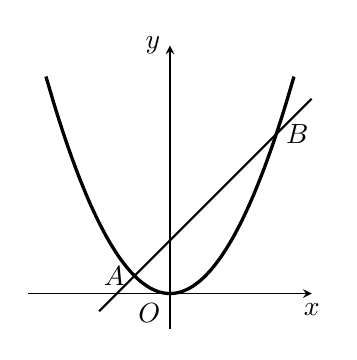
\begin{tikzpicture}[>=stealth, scale=.45]
    \draw[->](-4,0)--(4,0)node[below]{$x$};
    \draw[->](0,-1)--(0,7)node[left]{$y$};
    \node[below left]{$O$};
    \draw[domain=-3.5:3.5, smooth, very thick]plot(\x, 0.5*\x*\x);
    \draw[thick](-2,-.5)--(4,5.5);
    \node at (-1,.5)[left]{$A$};
    \node at (3,4.5)[right]{$B$};
\end{tikzpicture}
\captionof{figure}{}
\end{minipage}

所以公共点$A$、$B$的坐标分别是$\left(-1,\; \frac{1}{2}\right)$、$\left(3,\; \frac{9}{2}\right)$. 直线被曲线截得的线段长
\[|AB|=\sqrt{(3+1)^2+\left(\frac{9}{2}-\frac{1}{2}\right)^2}=4\sqrt{2}\]
\end{solution}

\begin{example}
已知某圆的方程是$x^2+y^2=2$. 当$b$为何值时，直线$y=x+b$与圆有两个公共点；一个公共点；没有公共点？
\end{example}

\begin{solution}
解方程组$\begin{cases}y=x+b& (1)\\x^2+y^2=2 &(2)\end{cases}$
把(1)式代入(2)式，得
\begin{align}
x^{2}+(x+b)^{2}&=2 \nonumber\\
2x^{2}+2bx+b^{2}-2&=0    \tag{3}
\end{align}

\noindent
\begin{minipage}{.45\textwidth}
\CTEXindent 方程(3)的根的判别式
\[\begin{split}
    \Delta&=(2b)^{2}-4\cdot2(b^{2}-2)\\
    &=4(-b^{2}+4)\\
    &=4(2+b)(2-b)
\end{split}\]

当$-2<b<2$时，$\Delta>0$, 方程组有两个不同的实数解，直
线与圆有两个公共点；

当$b=\pm2$时，$\Delta=0$, 方程组有一个实数解，因此直线与圆有一个公共点；

当$b<-2$或$b>2$时，$\Delta<0$, 这时方程组没有实数解，因
此直线与圆没有公共点.    
\end{minipage}\hfill
\begin{minipage}{.5\textwidth}
\centering
\begin{tikzpicture}[>=stealth]
    \draw[->](-3,0)--(3,0)node[below]{$x$};
    \draw[->](0,-3)--(0,3)node[left]{$y$};
    \node[below right]{$O$};
\draw(0,0) circle(1);
\draw[domain=-2:.5, smooth]plot(\x, \x+1.414);
\draw[domain=-.5:2, smooth]plot(\x, \x-1.414);
\draw[domain=-1.5:1, smooth, dashed]plot(\x, \x+1.414/2);
\draw[domain=-1:1.5, smooth, dashed]plot(\x, \x-1.414/2);
\draw[domain=-1.25:1.25, smooth, dashed]plot(\x, \x);
\draw[domain=-.5:2.5, smooth, dashed]plot(\x, \x-1.414*3/2);
\draw[domain=-2.5:.5, smooth, dashed]plot(\x, \x+1.414*3/2);
\end{tikzpicture}
\captionof{figure}{}
\end{minipage}


实际上，上述三种情况，就是直线与圆相交、相切、相
离(图1.20).
\end{solution}

\begin{ex}
\begin{enumerate}
    \item \begin{enumerate}[(1)]
        \item 已知曲线$C$是以原点$O$为圆心，以2为半径的半圆（如图），试问$x^2+y^2=4$是否是曲线$C$的方程，并说明理由.
        \item 已知曲线$L$是一条抛物线（如图），试问方程$x=\sqrt{y}$是曲线$L$的方程吗？说明理由.
    \end{enumerate}
\begin{center}
\begin{tikzpicture}[>=stealth]
\begin{scope}
    \draw[->](-1,0)--(2,0)node[below]{$x$};
    \draw[->](0,-2)node[below]{第1(1)题}--(0,2)node[left]{$y$};
    \node[below left]{$O$};
\draw(0,1.25) arc (90:-90:1.25);
\node at (1.25,0)[below right]{2};
\end{scope}
\begin{scope}[xshift=5cm, yshift=-1cm]
    \draw[->](-2,0)--(2,0)node[below]{$x$};
    \draw[->](0,-1)node[below]{第1(2)题}--(0,3)node[left]{$y$};
    \node[below left]{$O$};
\draw[domain=-1.5:1.5, smooth, samples=100, thick]plot(\x, \x*\x);
\draw[dashed](-1,0)node[below]{$-1$}--(-1,1)--(0,1)node[above right]{1}--(1,1)--(1,0)node[below]{1};
\end{scope}
\end{tikzpicture}
\end{center}

\item 点$A(1,-2)$、$B(2,-3)$、$C(3,10)$是否在曲线
$x^2-xy+2y+1=0$上？
\item \begin{enumerate}[(1)]
\item 在什么情况下，曲线$y=ax^2+bx+c$经过原点和$P(1,1)$点？
\item 在什么情况下，曲线$(x-a)^2+(y-b)^2=r^2$经过原点？
\end{enumerate}

\item 求直线$2x-5y+5=0$与曲线$y=\frac{-10}{x}$的公共点.
\end{enumerate}
\end{ex}

\section{曲线与方程的两个基本问题}
从理论上或实践中，经常遇到的曲线与方程的两个基本问题是：（1）给一条曲线，求出它的方程，并且用方程研究这条曲线的性质；（2）给一个方程，画出它的曲线，并且用曲线研究这个方程的解.第一个问题实质上是把曲线转化为它的代数形式——方程，然后用代数方法研究曲线；第二个
问题实质上是把方程转化为它的几何形式，然后用几何方法研究方程的解，它属于解析几何在代数上的应用.

前面已经指出，以集合论的观点，曲线可以看作是具有某种本质特征（条件）的点的集合，或者看作是动点按照某种运动规律运动的轨迹.很明显，不论是集合的观点还是轨迹的观点，都意味着：
\begin{enumerate}[(1)]
\item 这条曲线上的点都具有这种本质特征（纯粹性）；
\item 具有这种本质特征的点都在这条曲线上（完备性）．
\end{enumerate}
由此可以得到：

点$P$在曲线$C$上$\Longleftrightarrow$点$P$具有曲线$C$上点的本质特征.

当我们说“已知曲线”，就是说知道曲线上点的共同的本质特征，或者说画出了这条曲线.

下面分别研究曲线与方程的两个基本问题.

\subsection{已知曲线，求曲线的方程}

我们先看下面的例子.

\begin{example}
 设$A$、$B$两点的坐标是$(-1,-1)$、$(3,7)$，求线段$AB$的垂直平分线的方程.
\end{example}

\begin{solution}
    设$M(x,y)$是线段$AB$的垂直平分线上任意一点（图1.21），也就是点$M$属于集合

    \noindent
\begin{minipage}{.6\textwidth}
\CTEXindent    \[P=\{M\mid |MA|=|MB|\}\]

由两点的距离公式，点$M$所适合的条件可表示为
\[\sqrt{(x+1)^2+(y+1)^2}=\sqrt{(x-3)^2+(y-7)^2}\]
两边平方后，得
\[(x+1)^2+(y+1)^2=(x-3)^2+(y-7)^2\]
即：$x+2y-7=0$. \hfill (1)

下面，我们证明方程(1)是线段$AB$的垂直平分线的方程.    
\end{minipage}\hfill
\begin{minipage}{.35\textwidth}
\centering
\begin{tikzpicture}[>=stealth, scale=.5]
\draw[->](-3,0)--(5,0)node[below]{$x$};
\draw[->](0,-2)--(0,8)node[left]{$y$};
\tkzDefPoints{-1/-1/A, 3/7/B, 1/3/C, -1/4/M}
\draw[thick](A)node[below]{$A$}--(B)node[right]{$B$};
\draw[thick](-3,5)--(3,2);
\draw[dashed](A)--(M)node[above]{$M$}--(B);
\node [below right]{$O$};
\end{tikzpicture}
\captionof{figure}{}
\end{minipage}

\begin{enumerate}[(1)]
\item 由上面求方程的过程可知，垂直平分线上每一点的坐标都是方程(1)的解；
\item 设点的坐标$(x_1,y_1)$是方程(1)的解，即
\[x_1+2y_1-7=0 \quad \Rightarrow\quad x_1=7-2y_1\]
点$M_1$到$A$、$B$的距离分别是
\[\begin{split}
|M_1A|=\sqrt{(x_1+1)^2+(y_1+1)^2}&=\sqrt{(8-2y_1)^2+(y_1+1)^2}\\
&=\sqrt{5(y^2_1-6y_1+13)}\\
|M_1B|=\sqrt{(x_1-3)^2+(y_1-7)^2}&=\sqrt{(4-2y_1)^2+(y_1-7)^2}\\
&=\sqrt{5(y^2_1-6y_1+13)}\\
\end{split}\]
$\therefore\quad |M_1A|=|M_1B|$
即点$M_1$在线段$AB$的垂直平分线上．
\end{enumerate}
\end{solution}

由上述证明可知，方程(1)是线段$AB$的垂直平分线的方程.

由上面的例子可以看出，求曲线（图形）的方程，一般有下面几个步骤：
\begin{enumerate}[(1)]
\item 建立适当的直角坐标系，用$(x,y)$表示曲线上任意一点$M$的坐标；
\item 写出适合条件$p$的点$M$的集合$P=\{M\mid p(M)\}$;
\item 用坐标表示条件$p(M)$，列出方程$f(x,y)=0$;
\item 化方程$f(x,y)=0$为最简形式；
\item 证明以化简后的方程的解为坐标的点都是曲线上的点.
\end{enumerate}

如果化简过程是同解变形过程，步骤（5）可以省略不写，如有特殊情况，可适当予以说明. 另外，根据情况，也可以省略步骤（2），直接列出曲线方程．

\begin{example}
  设两定点$F_1$、$F_2$的距离是8，求到$F_1$和$F_2$的距离的平方和是50的动点运动的轨迹方程.
\end{example}

\begin{solution}
\textbf{解法1：}
以$F_1$、$F_2$的连线为$x$轴，以$F_1F_2$的垂直平分线为$y$轴建立坐标系（图1.22），
则$F_1$、$F_2$的坐标分别为$(-4,0)$和$(4,0)$. 设$P(x,y)$为曲线（轨迹）上任意一点，则
\[|PF_1|^2+|PF_2|^2=50\]

根据两点间距离公式，上式表达的几何条件转化为代数形式，得
\[\left[\sqrt{(x+4)^2+y^2}\right]^2+\left[\sqrt{(x-4)^2+y^2}\right]^2=50\]
化简，得：$x^2+y^2=9$.\hfill (2)

\noindent
\begin{minipage}{.45\textwidth}
\centering
\begin{tikzpicture}[>=stealth, scale=.4]
    \draw[->](-6,0)--(6,0)node[below]{$x$};
    \draw[->](0,-5)--(0,6)node[left]{$y$};
\node[below left]{$O$};
\draw[thick](0,0) circle (3);
\tkzDefPoints{-4/0/F_1, 4/0/F_2}
\tkzDefPoint(60:3){P}
\draw[thick](F_1)node[above left]{$F_1(-4,0)$}--(P)node[above right]{$P(x,y)$}--(F_2)node[above right]{$F_2(4,0)$};
\foreach \x in {-4,4}
{
    \node at (\x,0)[below]{$\x$};
}
\node at (0,3)[above right]{$3$};
\node at (0,-3)[below right]{$-3$};


\end{tikzpicture}
\captionof{figure}{}
\end{minipage}\hfill
\begin{minipage}{.45\textwidth}
\centering
\begin{tikzpicture}[>=stealth, scale=.4]
    \draw[->](-6,0)--(6,0)node[below]{$x$};
    \draw[->](-4,-5)--(-4,6)node[left]{$y$};
    \draw[thick](0,0) circle (3);
    \tkzDefPoints{-4/0/F_1, 4/0/F_2}
    \tkzDefPoint(120:3){P}
\draw[thick](F_1)node[below left]{$F_1(O)$}--(P)node[above]{$P(x,y)$}--(F_2)node[above right]{$F_2(8,0)$};
\foreach \x in {4,8}
{
    \draw(\x-4,0)node[below]{\x}--(\x-4,.2);
}

    
\end{tikzpicture}
\captionof{figure}{}
\end{minipage}



\begin{proof}
\begin{enumerate}[(1)]
\item 由上面求方程的过程可知，到$F_1$和$F_2$的距
离的平方和是50的每一点的坐标都是方程(2)的解．
\item 由于化简过程是方程同解变形过程，因此可知，坐标满足方程(2)的点到$F_1$和$F_2$的距离的平方和是50，所以此点在轨迹上.

$\therefore\quad $所求轨迹方程是
$x^2+y^2=9$.
\end{enumerate}
\end{proof}

\textbf{解法2：}
以$F_1$、$F_2$的连线为$x$轴，以过$F_1$且垂直$F_1F_2$的直线为$y$轴建立坐标系（图1.23），则$F_1$、$F_2$的坐标分别是$(0,0)$、$(8,0）$，设动点为$P(x,y)$，则$|PF_1|^2+|PF_2|^2=50$. 

把$|PF_1|$和$|PF_2|$转化成代数形式，可得
\[\left(\sqrt{x^2+y^2}\right)^2+\left(\sqrt{(x-8)^2+y^2}\right)^2=50\]
化简，得：$x^2+y^2-8x+7=0$

证明的第二步可利用化简过程是方程同解变形过程进行证明，也可直接证明，即设$(x_0,y_0)$的坐标满足方程，有$x_0^2+y_0^2-8x_0+7=0$，然后推导出$|MF_1|^2+|MF_2|^2=50$，读者可以试一试.
\end{solution}

\begin{remark}
    解法1和解法2由于选择的坐标系不同，因此对同一轨迹得到的方程形式也不同. 这里，就需要选择适当的坐标系，使求曲线的方程过程变得简单，或使所得曲线方程的形式简单.
\end{remark}
 
\begin{example}
已知两点$A(-2,-2)$，$B(2,2)$，试求满足条件$|MA|-|MB|=4$的动点$M$的轨迹方程.
\end{example}
    
\begin{solution}
    设动点$M$的坐标为$(x,y)$，则由条件$|MA|-|MB|=4$可得：
\[\sqrt{(x+2)^2+(y+2)^2}-\sqrt{(x-2)^2+(y-2)^2}=4\]
移项得：
\[\sqrt{(x+2)^2+(y+2)^2}=\sqrt{(x-2)^2+(y-2)^2}+4\]
两边平方，整理得
\begin{equation}
    \sqrt{(x-2)^2+(y-2)^2}=x+y-2 \tag{3}
\end{equation}

当$x+y-2\ge 0$时，两边平方，整理得
\begin{equation}
    xy=2\qquad (x+y-2\ge 0) \tag{4}
\end{equation}
证明留给读者.
\end{solution}

\begin{remark}
    为什么要附加条件$x+y-2\ge 0$？因为在此条件
    下，方程化简变形是同解变形，从而保证方程(4)是轨迹的方程.若不加条件$x+y-2\ge 0$，很显然，由(3)变形到(4)是一增根过程，例如
    $P(-1,-2)$的坐标满足方程(4)而不满足方程(3)，因此$P$不是轨迹上的点. 附加条件$x+y-2\ge 0$, 从代数意义上讲，是在方程$xy=2$的解集中除去满足$x+y-2<0$的
    那些解，因为这些解不是方程(3)的解. 其几何意义是，在反 比例函数$y=\frac{2}{x}$的图象上除去使$x+y-2<0$的部分——图1.24用虚线画出的那一支曲线．
\end{remark}

\begin{figure}[htp]
    \centering
\begin{tikzpicture}[>=stealth, scale=.6]
    \draw[->](-4,0)--(5,0)node[below]{$x$};
    \draw[->](0,-4)--(0,5)node[left]{$y$};
\node[below left]{$O$};
\draw[domain=.5:4, smooth, thick]plot(\x, 2/\x);
\draw[domain=.5:4, smooth, dashed]plot(-\x, -2/\x);
\foreach \x in {-2,2}
{
    \draw(\x,0)node[below]{$\x$}--(\x,.2);
}
\draw(0,2)node[left]{2}--(0.2,2);
\draw(0,-2)--(0.2,-2)node[right]{$-2$};
\tkzDefPoints{2/2/B, -2/-2/A, .667/3/M}
\draw[very thick](A)node[below]{$A(-2,-2)$}--(M)node[above right]{$M(x,y)$}--(B)node[right]{$B(2,2)$};

\end{tikzpicture}
    \caption{}
\end{figure}

由此可见，化简方程时，保证同解变形对求曲线方程是十分重要的.

\subsection{已知曲线的方程，画出曲线}
这个问题我们将在第三章做些研究.


\begin{ex}
\begin{enumerate}
    \item 已知点$M$到$x$轴、$y$轴的距离的乘积等于1，求点$M$的轨迹方程.
    \item  已知点$M$与$x$轴的距离和它与点$F(0,4)$的距离相等，求点$M$的轨迹方程.
    \item  动点$P$到定点$A$、$B$的距离比为$2:1$，且$AB=2a$，求$P$点的轨迹方程.
\end{enumerate}    
\end{ex}

\section*{习题二}
\begin{center}
    \bfseries A
\end{center}

\begin{enumerate}
    \item 曲线$ax^2+by^2=4$过点$A(0,-2)$、$B\left(\frac{1}{2},\; \sqrt{3}\right)$，求$a$、$b$的值.
    \item 直线$y=kx+3$与曲线$\frac{x^2}{9}+\frac{y^2}{4}=1$有公共点，试确定$R$的取值范围.
    \item 点$P$到点$A(4,0)$的距离等于它到$y$轴的距离，求点$P$的轨迹方程.
    \item 点$M$到点$A(4,0)$和点$B(-4,0)$的距离的和为12，求点
    $M$的轨迹方程.
\end{enumerate}

\begin{center}
    \bfseries B
\end{center}

\begin{enumerate}\setcounter{enumi}{4}
    \item 点$M$到定点$F$的距离和它到定直线$L$的距离相等，且定点$F$到定直线$L$的距离为4，求点$M$的轨迹方程．
    \item 两根杆分别绕着定点$A$和$B$（$AB=2a$）在平面内转动，并且转动时两杆保持相互垂直，求杆的交点$P$的轨迹方程.
    \item  点$M$到点$F_1(-3,0)$和点$F_2(3,0)$的距离的差为4，求点$M$的轨迹方程.
\end{enumerate}

\begin{figure}[htp]
    \centering
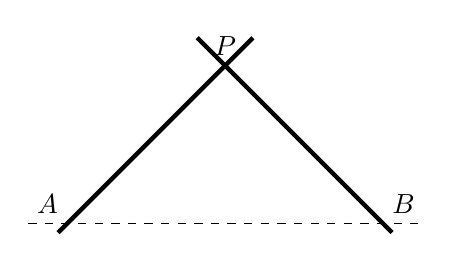
\begin{tikzpicture}
\draw[dashed](-2.5,-2)--(2.5,-2);
\draw[ultra thick](45:.5)--(-90-45:3);
\draw[ultra thick](90+45:.5)--(-45:3);
\node at (0,0)[above]{$P$};
\node at (-2,-2)[above left]{$A$};
\node at (2,-2)[above right]{$B$};


\end{tikzpicture}
    \caption*{第6题}
\end{figure}

\begin{center}
    \bfseries C
\end{center}

\begin{enumerate}\setcounter{enumi}{7}
    \item 用图解法判断方程$x^2-1-\frac{1}{x}=0$有无实数解？有几个？
    \item 两曲线的方程为$y=2x^2-1$、$x^2+y^2=r^2\; (r>0)$，
\begin{enumerate}[(1)]
\item 当$r$为何值时，两曲线有四个、三个、两个公共点和无公共点？
\item 这两曲线有可能只有一个公共点吗？试证明你的结论.
\end{enumerate}
\end{enumerate}